\noindent

\includegraphics[height=1.25cm]{images/pictograms/replication}

\includegraphics[height=1.25cm]{images/pictograms/benchmark}

\includegraphics[height=1.25cm]{images/pictograms/under_construction}
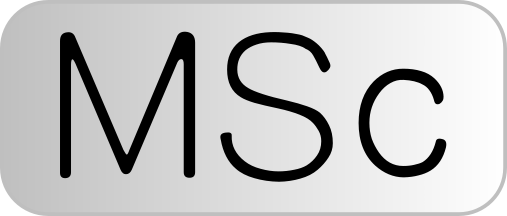
\includegraphics[height=1.25cm]{images/pictograms/msc}

\includegraphics[height=1.25cm]{images/pictograms/FEM}

\includegraphics[height=1.25cm]{images/pictograms/FDM}
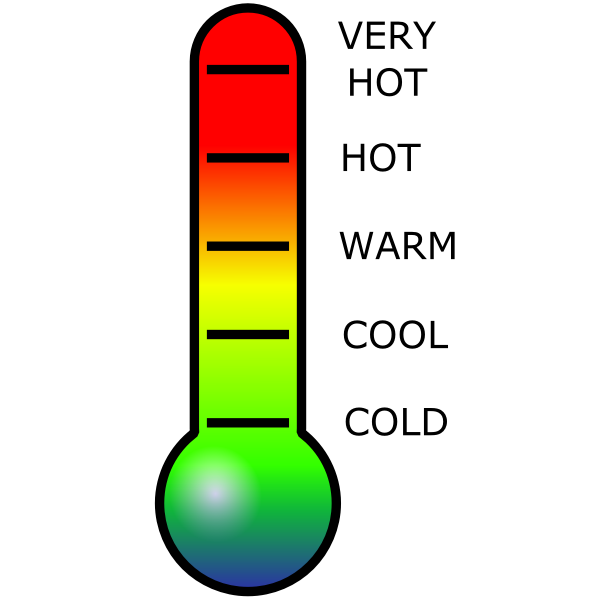
\includegraphics[height=1.25cm]{images/pictograms/temperature}

%%%%%%%%%%%%%%%%%%%%%%%%%%%%%%%%%%%%%%%%%%%%%%%%%%%%%%%%%%%%%%%%%%%%%%%%%%%%%%%%%%%%%%%%%%%%%%%%%%%

\begin{flushright} {\tiny {\color{gray} python\_codes/fieldstone\_169/text.tex}} \end{flushright}

%\lstinputlisting[language=bash,basicstyle=\small]{python_codes/template_keywords.key}

\par\noindent\rule{\textwidth}{0.4pt}

\begin{center}
\inpython
{\small Code: \url{https://github.com/cedrict/fieldstone/tree/master/python_codes/fieldstone_169}}
\end{center}

\par\noindent\rule{\textwidth}{0.4pt}

%{\sl This stone was developed in collaboration with Donald Duck}. \index{contributors}{D. Duck}

%\par\noindent\rule{\textwidth}{0.4pt}

%%%%%%%%%%%%%%%%%%%%%%%%%%%%%%%%%%%%%%%%%%%%%%%%%%%%%%%%%%%%%%%%%%%%%%%%%%%%%%%%%%%%%%%%%%%%%%%%%%%

This is an attempt at replicating the publication by \fullcite{stuw95}. 
When replicating a study I always first reproduce the abstract to give context:
\begin{displayquote}
{\color{darkgray}
A simple thermal model is used to investigate to what extent buffering effects 
of latent heat of fusion may prolong the thermal evolution of a one-dimensional, 
statically cooling, partially or completely melted heat source.
For a melting model appropriate for crustal rocks, the time of cooling of rocks 
through the solidus may be about tripled by this process. Depending on the melting 
model, cooling may halt completely near the solidus for time spans
comparable to the thermal time constant of the heat source.\\
In order to test the influence of this buffering effect on the equilibration of 
partially melted metamorphic rocks, these thermal model results are coupled with 
a simple diffusion model that relates the degree of equilibration of a
simple assemblage to temperature and cooling rate. It is shown that, for a broad 
range of initial heat source temperatures, freezing of selected mineral equilibria 
may occur in a comparably narrow temperature range at and
around the solidus. The calculations may have some relevance to low-P high-T 
metamorphic terranes in as much as they may provide an explanation for the widely 
observed equilibration and partial re-equilibration of rocks near the
crystallisation temperatures of partial melts.}
\end{displayquote}

\newpage
%==============================================================================
\section*{Theory}

The cooling history of an intrusion is described by the
thermal relaxation of an initial one-dimensional,
step-shaped temperature distribution

This initial condition may be described by $T=T_b$ in the region
$|z|>d/2$ and $T=T_i$ in the region $|z|<d/2$
where $T_b$ is the background temperature,
$T_i$ is the intrusion temperature, $d$ is the intrusion
thickness and $z$ is the distance from the intrusion centre. 
\begin{small}
\begin{verbatim}
                  Tb             Ti         Ti           Tb
          ------------------+----------+----------+-------------------> 
                          -d/2         0         d/2                  z
\end{verbatim}
\end{small}

For this initial condition, and if no latent
heat is considered, the thermal energy balance
can be solved analytically to give temperature as
a function of time, $t$, and distance by \cite{jaeg64}:
\begin{equation}
T(z,t)=T_b + \frac{T_i-T_b}{2} 
\left(
\text{erf} \left( \frac{d/2 +z}{\sqrt{4\kappa t}} \right)
+
\text{erf} \left( \frac{d/2 -z}{\sqrt{4\kappa t}} \right)
\right)
\label{eq:f169ana}
\end{equation}
where $\kappa$ is the thermal diffusivity.


For the thermal parameters we use average
values appropriate to the Earth's crust that are
commonly used in the literature:
$\rho=2800~\si{\kg\per\cubic\meter}$, $k=2.5~\si{\watt\per\meter\per\kelvin}$, $C_p=1100~\si{\joule\per\kg\per\kelvin}$.
Both $C_p$ and $k$ are assumed to be independent of
temperature\footnote{Although not made explicit in the 
paper so is density} 
so that they can be combined into the thermal 
diffusivity $\kappa=8.11688\cdot10^{-7}~\si{\square\meter\per\second}$.
For the latent heat of fusion a value
of $L = 320~\si{\kilo\joule\per\kg}$ is assumed. Parameter space
is explored for intrusions of thicknesses $d = 20 - 100~\si{\km}$, 
intrusion temperatures $T_i = 600-1000~\si{\celsius}$
and ambient background temperatures of $T_b =400~\si{\celsius}$. 


\begin{center}
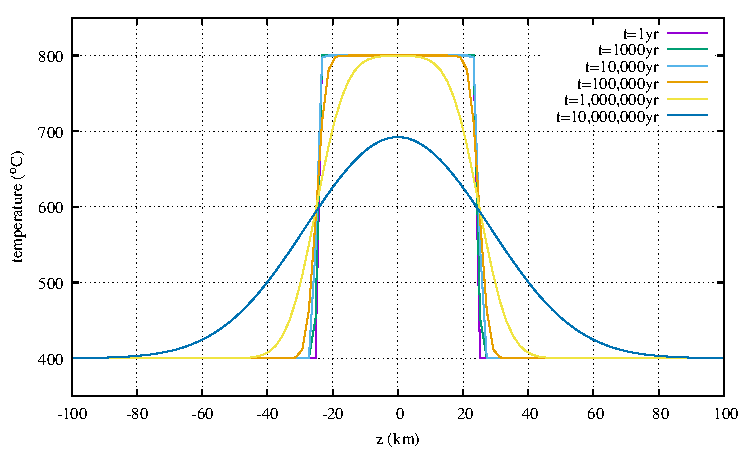
\includegraphics[width=10cm]{python_codes/fieldstone_169/images/solution.pdf}\\
{\captionfont Plot obtained 
with Eq.~\eqref{eq:f169ana}
for $T_b=400~\si{\celsius}$, $T_i=800~\si{\celsius}$ and $d=50~\si{\km}$.}
\end{center}


For many geological purposes it is useful to look at the
temperature-cooling-rate evolution rather than at
the temperature-time evolution. For the latent
heat absent case, this may be found by differentiating the equation above 
with respect to time so that the cooling rate, $s$, is given by {\color{red} check the maths}:
\[
s(z,t) = \frac{\partial T}{\partial t}
=-\frac{T_i-T_b}{4\sqrt{\pi \kappa t^3}}
\left(
\frac{d/2 +z}{\exp((d/2+z)^2/4\kappa t )}
+
\frac{d/2 -z}{\exp((d/2-z)^2/4\kappa t )}
\right)
\]

\begin{center}
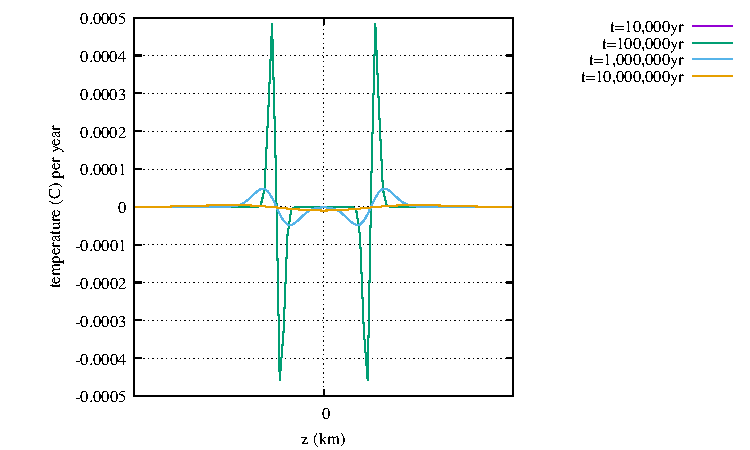
\includegraphics[width=10cm]{python_codes/fieldstone_169/images/solution_derv.pdf}\\
{\captionfont Plot obtained for $T_b=400~\si{\celsius}$, $T_i=800~\si{\celsius}$ and $d=50~\si{\km}$.}
\end{center}


Melting of multi-component metamorphic rocks is likely to occur between a solidus
temperature, $T_s$, and a liquidus temperature, $T_l$.
Between these two temperatures melting is likely
to occur along a series of melt producing reactions but details of the melt volume-temperature
relationships are poorly understood, in part because they depend on a range of ill-constrained
variables, for example, the presence of a fluid
(e.g., Vielzeuf and Holloway, 1988). Here a simple model function of the form:
\begin{equation}
v(T) = \frac{\exp(\alpha T)- \exp(\alpha T_s) }{\exp(\alpha T_l) - \exp(\alpha T_s) }
\label{eq:stuw95_eq3}
\end{equation}
is used in which the rate of melt production between $T_s$ and $T_l$ can be controlled by varying $\alpha$.
Obviously, when $T\rightarrow T_s$ then $v \rightarrow 0$ (no melt) while when
when $T\rightarrow T_l$ then $v \rightarrow 1$ (100\% melt).


For the melting model, a solidus temperature of $T_s=600~\si{\celsius}$ and a 
liquidus temperature of $T_l = 1200~\si{\celsius}$ are assumed.


\begin{center}
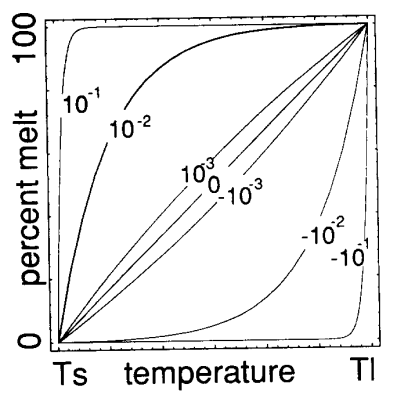
\includegraphics[width=6cm]{python_codes/fieldstone_169/images/stuw95a}
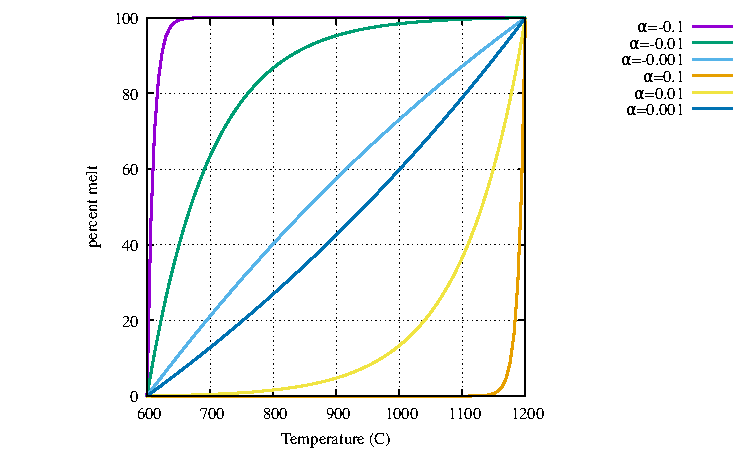
\includegraphics[width=10cm]{python_codes/fieldstone_169/images/percent_melt}\\
Left: plot (taken from the paper) of melt volume against temperature taken as given by
the melting model of Eq.~\eqref{eq:stuw95_eq3}. Different melting models may
be explored by varying the parameter $\alpha$, for which the diagram 
is contoured. In most of the following calculations
$\alpha= - 0.01$ is used (thick line).
Right: my own version of the plot. {\color{red} There is an obvious sign issue with the labels}.
\end{center}



For positive $\alpha$ most of the melt production occurs near $T_l$, for negative a most of the
melt production occurs near $T_s$ (This seems to agree with my plot rather than the 
one in the paper?). For this melting
model the thermal energy balance may not be
solved analytically and a finite difference scheme
was employed to obtain numerical solutions in the article.

These solutions were obtained by incorporating the effects of latent heat into a modified heat
capacity (see the Appendix of the paper) and the results were back checked by
comparing them with the analytical solution of
Stefan (1891) for $T_i = T_l$ and large negative $\alpha$.

We start from the 1D heat transport equation with no advection term:
\[
\rho C_p \frac{\partial T}{\partial t} + \rho L \frac{\partial v}{\partial t} 
= k  \frac{\partial^2 T}{\partial z^2} 
\]
where $\partial v/ \partial t$ describes the change in the proportion of melt with time.
as it is assumed that the intrusion is not completely molten, but that the
melt percentage at $T_i$ is given by Eq.~\eqref{eq:stuw95_eq3}.

In order to solve this equation it is useful to replace:
\[
\frac{\partial v}{\partial t} = \frac{\partial v}{\partial T}\frac{\partial T}{\partial t}
\]
so that now the heat transport PDE is given by
\[
\rho C_p \frac{\partial T}{\partial t} + \rho L 
\frac{\partial v}{\partial T}\frac{\partial T}{\partial t}
= k  \frac{\partial^2 T}{\partial z^2} 
\]
or,
\[
\rho \left(C_p + L \frac{\partial v}{\partial T} \right)
\frac{\partial T}{\partial t} = k  \frac{\partial^2 T}{\partial z^2} 
\]
and finally, what we call option 1:
\[
\boxed{
\rho \underbrace{\left(C_p + L \frac{\partial v}{\partial T} \right)}_{C_p(T)}
\frac{\partial T}{\partial t} = k  \frac{\partial^2 T}{\partial z^2} 
}
\]
or, what we will call option 2:
\[
\boxed{
\frac{\partial T}{\partial t} = 
\underbrace{\frac{k}{\rho \left(C_p + L \frac{\partial v}{\partial T} \right)}}_{\kappa(T)} \frac{\partial^2 T}{\partial z^2} 
}
\]
Both are nonlinear 1D diffusion equations.  The second approach 
is taken in the paper (see Eq.~8, obtained with FDM).
In passing, let us note that the author 
1) does not mention boundary conditions at all,
2) uses an explicit time discretisation,
3) does not elaborate about how he deals with the nonlinearities.    
concerning the boundary conditions, all what we have to do is 
consider a domain large enough so 
as to avoid boundary effects and prescribe $T_b$ on both ends.

When discretised using FEM, we will obtain the following system:
\[
\M \cdot \dot{\vec{{\cal T}}} + \K_d \cdot \vec{\cal T} = 0
\]
In option 1 the mass matrix $\M$ is nonlinear while the diffusion matrix $\K_d$ is linear.
In option 2 the mass matrix $\M$ is linear while the diffusion matrix $\K_d$ is nonlinear.

When discretised using FDM and resorting to an explicit scheme we will
naturally adopt option 2.

From Eq.~\eqref{eq:stuw95_eq3} we find that
\[
\frac{\partial v}{\partial T}  
= \frac{\alpha \exp (\alpha T) }{\exp(\alpha T_l) - \exp(\alpha T_s) } 
=A \exp (\alpha T)
\]
so that the heat diffusion coefficient for option 2 is then given by
\[
\kappa(T) = \frac{k}{\rho \left(C_p + L A \exp(\alpha T) \right)}
\]
which is only valid for temperatures between $T_s$ and $T_l$.


\begin{center}
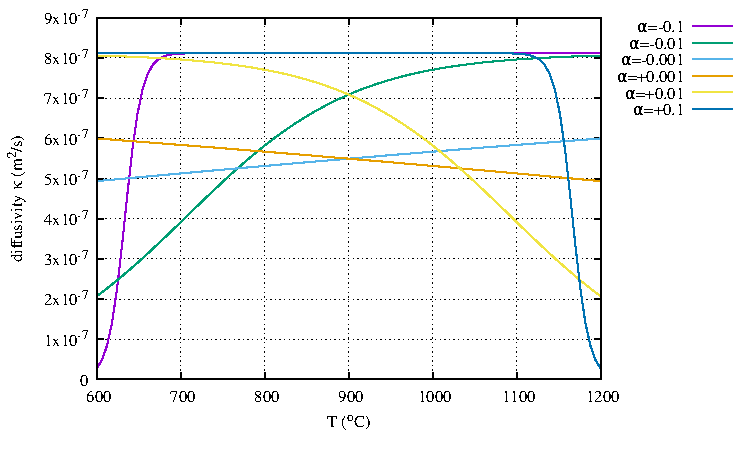
\includegraphics[width=10cm]{python_codes/fieldstone_169/images/kappa.pdf}
\end{center}
We find that the value of $\alpha$ can alter the value of $\kappa$ by almost an order of magnitude.

At this stage we can make a few remarks
\begin{enumerate}
\item melt not moving
\item matrix not deforming
\item 1D system implying infinite extent in $x,y$ direction
\end{enumerate}


%==========================================================
\section*{Discretisation and implementation}

%----------------------------------------------------------
\subsection*{Linear case (no melting)}

We adopt here a very simple approach, a forward in time, 
centered in space approach (FTCS) as explained in Section~\ref{MMM-ss:fdm_diff1D}. 
Except for the nodes on the boundary (where the temperature
is prescribed to be $T_b$) we have the following explicit stencil:
\[
T_i^{n+1} 
= 
T_i^n + \frac{\kappa \delta t }{h^2} (T_{i+1}^n-2T_i^n+T_{i-1}^n)
\]
This translates as follows in the code:

\begin{lstlisting}
Time=0.
for n in range(0,nstep):
    Time+=dt
    for i in range (0,nnx):
        if i==0:
           Tnew[i]=Tleft
        elif i==nnx-1:
           Tnew[i]=Tright
        else:
           Tnew[i]=Told[i]+dt*kappa/h**2*(Told[i+1]-2*Told[i]+Told[i-1])
        #end if
    #end for
    Told[:]=Tnew[:]
#end for
\end{lstlisting}
We define the analytical solution function as follows:
\begin{lstlisting}
def analytical_solution(x,t):
    return Tb+(Ti-Tb)/2*\
           (\
           erf((d/2+x)/np.sqrt(4*kappa*t)) +\
           erf((d/2-x)/np.sqrt(4*kappa*t)) \
           )
\end{lstlisting}
The timestep value is computed by means of a CFL conditions:
\begin{lstlisting}
dt=CFL_nb*h**2/2/kappa
\end{lstlisting}
The initial temperature is prescribed as follows:
\begin{lstlisting}
Told=np.zeros(nnx,dtype=np.float64)
Told[:]=Tb
for i in range(0,nnx):
    if abs(x[i])<d/2: Told[i]=Ti
\end{lstlisting}


TODO:

- add latent heat, implement nonlinear scheme

- compare option 1,2



\newpage
%==========================================================
\section*{Results}

%----------------------------------------------------------
\subsection*{Linear case (no melting)}

I have run the code with the following parameters:
\begin{lstlisting}
nnx=501
nstep=10000
Lx=400e3
rho=2800
Cp=1100
k=2.5
L=350e3
Tb=400
Ti=800
Ts=600
Tl=1200
d=50e3
CFL_nb=0.1
tfinal=5e6*year
\end{lstlisting}
We find that the temperature field indeed follows the analytical solution:
\begin{center}
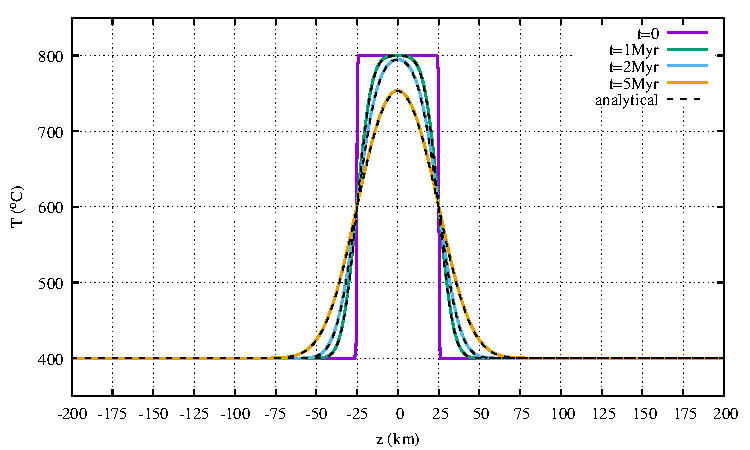
\includegraphics[width=12cm]{python_codes/fieldstone_169/results/linear/T.pdf}
\end{center}
The absolute error is only a few degrees at most:
\begin{center}
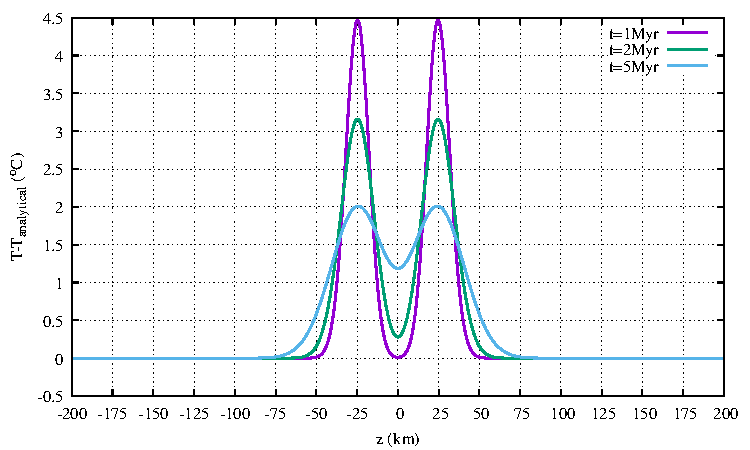
\includegraphics[width=12cm]{python_codes/fieldstone_169/results/linear/T_error.pdf}
\end{center}






